% =============================================================================
% FIGURE PLACEHOLDER - Phylogeny
% =============================================================================
% Placeholder for phylogenetic tree figure

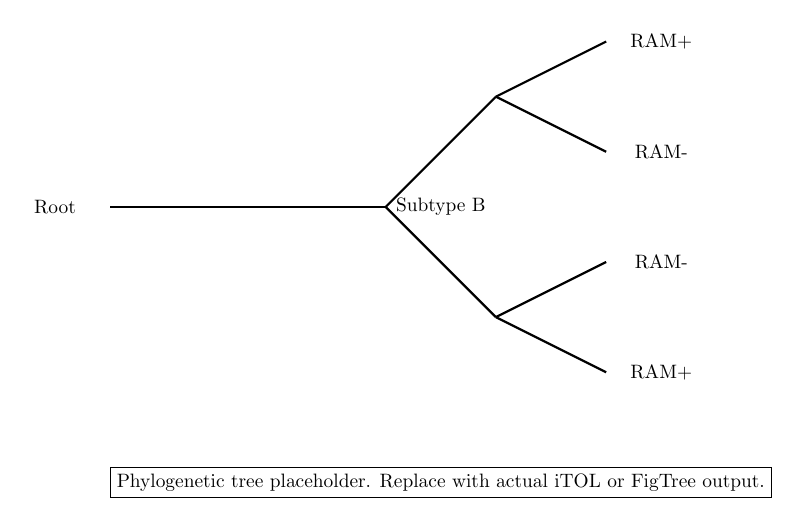
\begin{tikzpicture}[scale=0.7, transform shape]
    \draw[thick] (0,0) -- (5,0);
    \draw[thick] (5,0) -- (7,-2);
    \draw[thick] (5,0) -- (7,2);
    \draw[thick] (7,-2) -- (9,-3);
    \draw[thick] (7,-2) -- (9,-1);
    \draw[thick] (7,2) -- (9,1);
    \draw[thick] (7,2) -- (9,3);

    \node at (-1,0) {Root};
    \node at (6,0) {Subtype B};
    \node at (10,-3) {RAM+};
    \node at (10,-1) {RAM-};
    \node at (10,1) {RAM-};
    \node at (10,3) {RAM+};

    \node[draw, rectangle] at (6,-5) {Phylogenetic tree placeholder.
    Replace with actual iTOL or FigTree output.};
\end{tikzpicture}